% APPENDIX B
\newpage
\appendix

\section{Appendix B: GRACE methods of data reduction \label{app:b}}
\textbf{\textit{Adapted directly from} \textsc{Resolving and Contextualizing the Signal of Greenland Ice Loss 2014--2017}, \cite{getraerFall}, and \textsc{Regional Forcing of Greenland Ice Loss 2002--2017}, \cite{getraerSpring}}

{\it
The Gravity Recovery and Climate Experiment is a twin-satellite mission active
2002--2017, with its final data collection completed in October 2017. GRACE
measurements are made accessible in the form of several data products offered
through NASA and partnered agencies, which generally rely on a method of data
reduction to translate the ``Level~1'' GRACE measurements of satellite positions into globally projected mass anomaly estimations. There are two primary
methods of data reduction: The creation of ``mascons,'' roughly equal-area
sections around the globe on the scale of single arc-degrees, each assigned a
single number representing mass change, and the calculation of spherical
harmonic coefficients, which correspond to continuous functions in three
dimensions that when summed can model the spatially continuous variation of mass
on the surface of Earth. The difference between continuous and discrete data reduction (harmonics vs. mascons) often has to do with localization of the signal in time and space. Discrete solutions may not be able to ``see'' continuous large scale patterns, while continuous solutions necessarily ``hide'' information about very localized signals in a collection of globally continuous patterns.

The spherical harmonic method requires continuous functions on Earth's surface, whereby a field of interest can be developed into a series solution of
eigenfunctions $Y_{lm}(\theta,\phi)$, where $l$ refers to the ``order''
(integers $0$ to $\infty$) and $m$ the ``degree'' (integers $-l$ to $+l$) of
each harmonic ($\theta$ and $\phi$ reference location on the surface of Earth). Due
to limitations in computational power and in the spatial resolution of the data
being modeled by the harmonic functions, calculated solutions are bandlimited,
meaning that they are calculated up to a finite order $L$. See
\cite{Simons+2006a}, their section~3 for a concise summary. See our
Figure~\ref{fig:SlepvSH} for illustrations of low-order spherical harmonic
eigenfunctions.

\begin{figure}[h!]
\centering
\textbf{Comparison of Spherical Harmonic Eigenfunctions to Slepian Basis Eigentapers}\par\medskip
\includegraphics[height=0.5\textheight]
{/Users/benjamingetraer/Documents/IndependentWork/JuniorPaper/JP02/Figures/SlepvSH.pdf}
\caption[Comparison of Spherical Harmonic Eigenfunctions to Slepian Basis Eigentapers]{Three low-order spherical harmonic eigenfunctions $Y_{lm}(\theta,\phi)$ are illustrated in \textbf{A} as examples of the basic forms these functions take: zonal (left, $m=0$), sectoral (middle, $m=l$), and tesseral (right, $m\neq l\neq 0$). When expanded into a geographically-localized Slepian basis, the forms of these eigenfunctions have parallel eigentapers as illustrated in rows \textbf{B} and \textbf{C}. The eigentapers allow for reconstruction of a signal with power concentrated within a geographical basis, minimizing the effect of the signal outside of the basis on the series solution. $r$ is radius, $L$ is the bandlimit of maximum order $l$ used in the Slepian expansion.} \label{fig:SlepvSH}
\end{figure}

Monthly coefficients for bandlimited global spherical harmonic solutions of the
time-variable geopotential field are independently calculated by three different
processing centers (GFZ in Potsdam, Germany; CSR at University of Texas, Austin; JPL at
California Institute of Technology) and published publicly as the GRACE
Level~2 Release~05 products for a few different bandwidths (see
\nameref{app:a}). The RL05 product is pre-corrected to remove the time-invariant
geopotential field using the GRACE Gravity Model~03 \cite[][]{GGM032007}, and we
use coefficients describing Earth's center of mass \cite[spherical harmonic
degree~1, from][]{swenson2008} and oblateness \cite[spherical harmonic degree~2,
order~0, from][]{cheng2013} calculated from Satellite Laser Ranging in order to
accurately capture mass variations on scales much larger than the area covered
by the GRACE satellites (see \nameref{app:a}). The coefficients are released as contributions to gravitational potential in units of $\frac{kg^{2}}{s^{2}}$, and are converted to equivalent surface density on Earth in units of $\frac{kg}{m^{2}}$ using the method of \cite{wahr1998}. Mass estimates are calculated through area-integration, and converted to sea-level equivalence using the method of \cite{tian2015}.

A third method of data reduction uses the spherical harmonic coefficients in a linear combination of their respective functions to
constrain explanatory power to an arbitrary geographic location \cite[][]{Simons+2006a}.
This method generates linear combinations of the spherical harmonic
eigenfunctions $Y_{lm}(\theta,\phi)$ called scalar Slepian functions
$g_{\alpha}(\theta,\phi)$, where $\alpha$ refers to the ``rank'' of the Slepian
function, which is a single linear combination of all spherical harmonic
eigenfunctions up to order $L$, also referred to as an ``eigentaper.'' Formally, this expansion is expressed in terms of the spherical harmonic eigenfunctions by:
\begin{equation}\label{eq:sh}
\sum_{l=0}^{L}\sum_{m=-l}^{l}f_{lm}Y_{lm}(\theta,\phi)= 
\sum_{\alpha=1}^{(L+1)^{2}}f_{\alpha}g_{\alpha}(\theta,\phi)
\end{equation}
	By construction the functions $g_{\alpha}(\theta,\phi)$ are centered around the geographic region of interest. A few eigentapers are concentrated in power strictly within the region, and most are concentrated in power predominantly outside of the region. The signal within the region is approximated by choosing those functions $g_{\alpha}(\theta,\phi)$ whose ratio of power inside of that region to outside of the region is significant (often around $\geq\frac{1}{2}$), the number of which is referred to as the Shannon number $N$. The resulting spatially concentrated estimation of the global field is expressed in the approximation:
\begin{equation}\label{eq:sh2sf}
\sum_{l=0}^{L}\sum_{m=-l}^{l}f_{lm}Y_{lm}(\theta,\phi)\approx 
\sum_{\alpha=1}^{N}f_{\alpha}g_{\alpha}(\theta,\phi)
\end{equation}
Though limited by $N$, the Slepian expansion is useful by reducing the
unnecessary information in the global spherical harmonic coefficients --- namely,
the signal everywhere else in the world. The method of calculating
geographically constrained scalar Slepian functions from a bandlimited series of
spherical harmonics, as well as the relationship between the geographical area
and the Shannon number is described in mathematical detail by
\cite{Simons+2006a}. See our Figure~\ref{fig:SlepvSH} for illustrations of low-rank
Slepian eigentapers in an circular, axisymmetric basis and a Greenland basis.

Slepian-based harmonics have the advantage of continuous solutions as opposed to
the coarse rasterized solutions of mascons, with less of the noise and bias
associated with globally continuous spherical harmonics. The expansion of global
spherical harmonics into a localized Slepian basis of eigentapers allows for
locally constrained signals to be extracted from the continuous global GRACE
RL05 data product with less impact from noise or signals from other geographic
locations, a problem that reduces the precision of the standard spherical
harmonic method. We will find localized mass anomaly solutions using the Slepian
expansion method of data reduction from the GRACE CSR
RL05 $L=60$ spherical harmonic coefficients \citep[see][]{Harig+2012}.


%\begin{wrapfigure}{r}{0.5\textwidth} 
\begin{figure}
\centering
\makebox[\textwidth][c]{
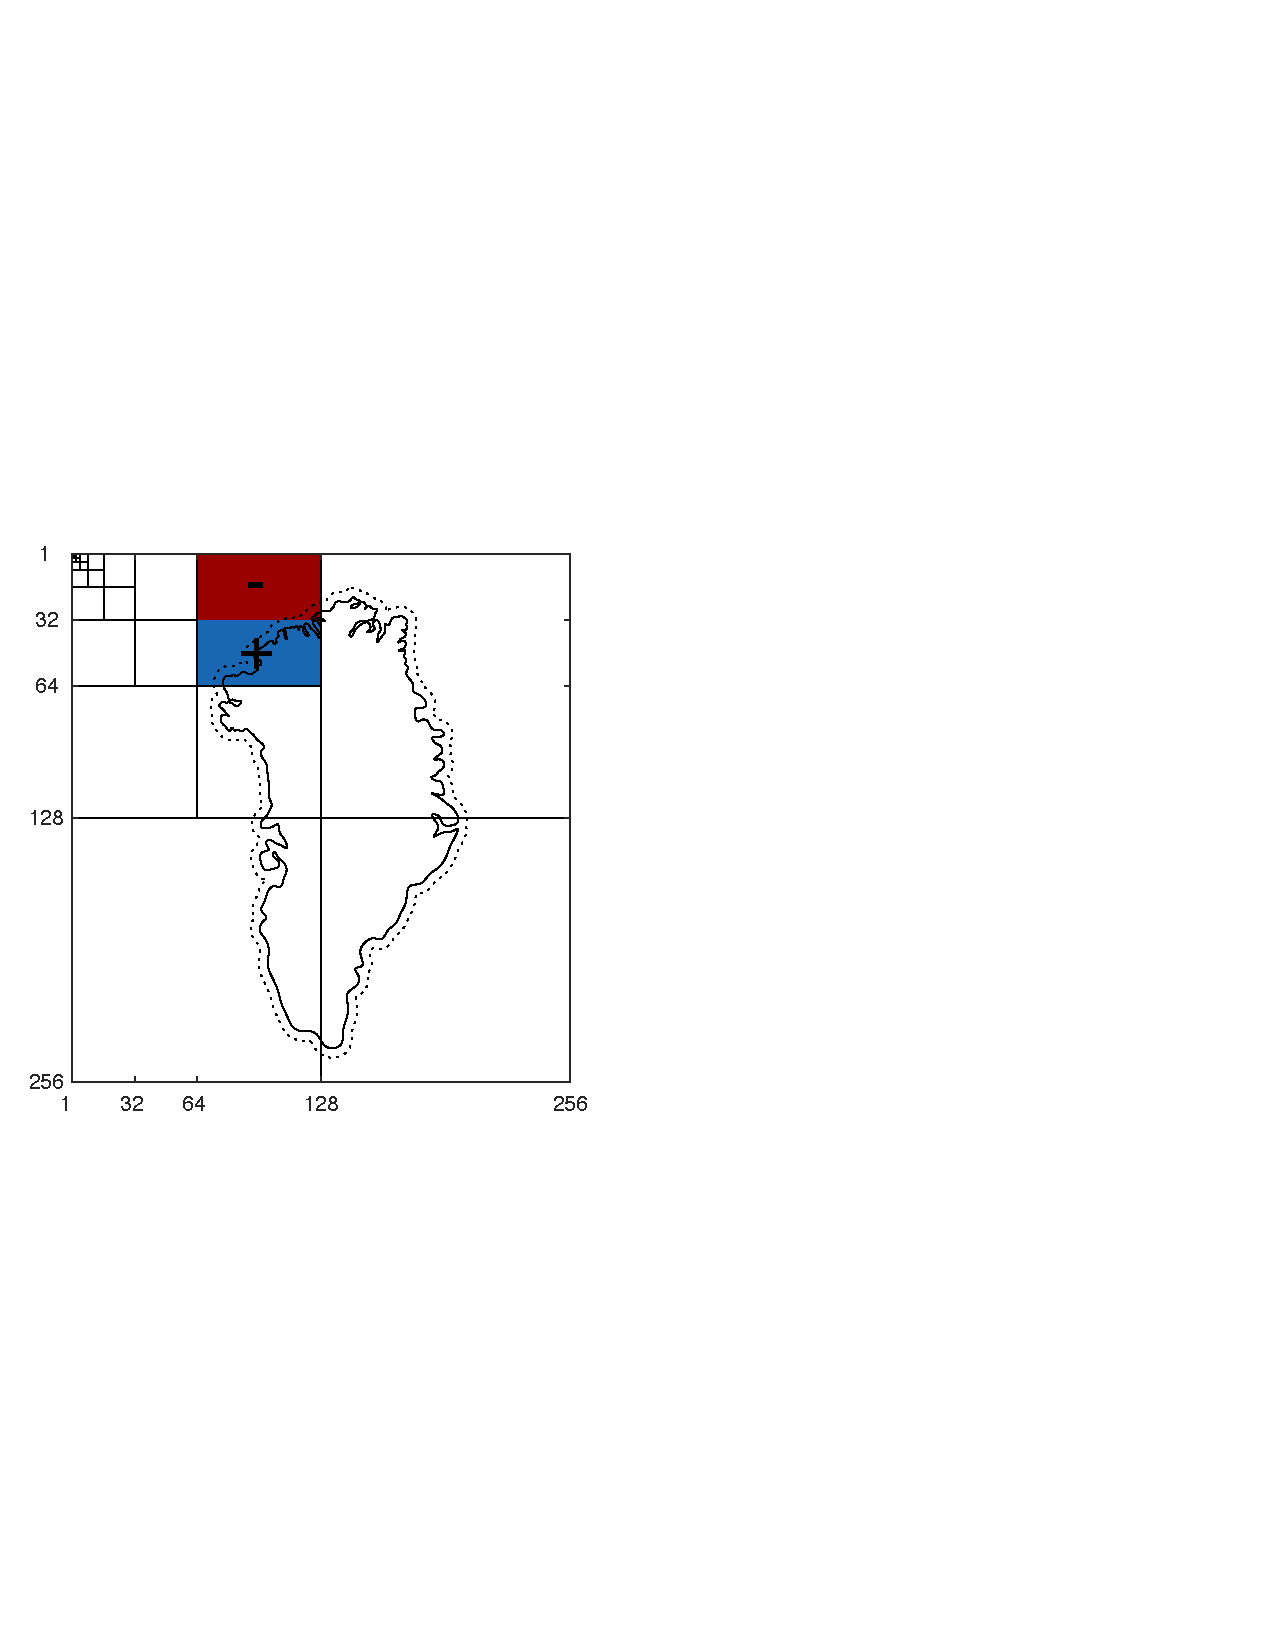
\includegraphics[width=0.5\linewidth]{/Users/benjamingetraer/Documents/IndependentWork/senior-thesis/figures/spring2019/wavemodel.pdf}}
\caption[The Wavelet Grid Around Greenland]{The grid extent around Greenland is defined in the global basis on a face of the \textit{Cubed Sphere} centered on Greenland \cite[see Figure~\ref{fig:gridbasins}~\textbf{A}~\&][]{ronchi1996}. In the image basis the grid is cartesian with length $256$. Grid lines in the image basis represent the diminishing areal support of wavelets of different levels, from $\zeta=8$ (the entire image) to $\zeta=1$ (a unit grid cell). Note that in reality, each wavelet level has coverage over the entire image. An example of a Haar wavelet basis function with discrete spatial support is shown in color. The dotted line around Greenland is a coastal buffer of $0.5^{\circ}$ as in Figure~\ref{fig:Getraer}~\& \cite{Harig+2016}.} \label{fig:thegrid}
%\end{wrapfigure}
\end{figure}

A fourth method of data reduction was explored in \cite{getraerSpring}, using 2-dimensional wavelet decomposition to define the spatial scales at which significant changes in mass loss were occurring in a specific area over a specific time-scale. Wavelets are oscillating functions with finite support in space. Wavelets of different scales capture signal at different resolution levels, and a discrete implementation of the transform would subsample a spatial grid depending on the scale. Each wavelet at each grid scale is assigned a weighting coefficient such that signal information at a location on the grid can be represented as a superposition of individual wavelets at different scale levels at that point. The weighting $m_{\beta}$ associated with the wavelet $w_{\beta}$ at each grid point, and at different scales of resolution, tells us where and how important information is at different scales (see Table~\ref{tab:exp_eq}~\& Figure~\ref{fig:thegrid}).



\begin{table}
\centering
\begin{tabular}{lll}
Approximation method & Expansion Equations & Spatial Support \\
\hline
Spherical Harmonic &  $\begin{aligned} M_{SH}(\underline{r}) = \sum_{l=0}^{L} \sum_{m=-l}^{+l} f_{lm} Y_{lm}(\underline{r}) \end{aligned}$ & global
\\
Slepian Functions & $\begin{aligned} M_{SF}(\underline{r}) = \sum_{\alpha=1}^{N} f_{\alpha} g_{\alpha}(\underline{r}) \end{aligned}$ & concentrated
\\
Wavelet Basis &  $\begin{aligned} M_{WB}(\underline{r}) = \sum_{\beta=1}^{K} m_{\beta} w_{\beta}(\underline{r}) \end{aligned}$ & compact
\end{tabular}
\caption[Expansion Equations for GRACE Data]{Expansions used to represent the mass density field $M(\underline{r})$. Note that each expansion is a superposition of a basis function (some $F_i(\underline{r})$) weighted by a constant (some $c_i$). The GRACE CSR RL05 spherical harmonic data have a bandwidth $L=60$, with a total of $(L+1)^2 = 3721$ coefficients required to describe the field in any point in space (see Equation~\ref{eq:sh}). In the Slepian expansion over Greenland, the Shannon number is $N\approx20$, a massive reduction in the coefficients needed to describe the field (see Equation~\ref{eq:sh2sf}). Finally, the wavelet basis is expanded on a square grid of length $\sqrt{K}$, where $K$ is the total number of wavelets in the complete expansion. By choosing wavelets by thresholded coefficient values and support within Greenland, we develop a partial wavelet reconstruction on a $256\times256$ grid over Greenland with only $68$ coefficients.\label{tab:exp_eq}}
\end{table}

The wavelet decomposition is defined on a square grid centered around Greenland (see Figure~\ref{fig:thegrid}). A single image, the difference between the mass density field at either end of the desired time-period (i.e. January 2003 -- June 2017), is used to develop a constrained wavelet basis, with the assumption that the most relevant spatial structures throughout the time-series will be apparent in the total difference from beginning to end. The discrete wavelet decomposition (analysis) and recomposition (synthesis) is a lossless transformation, however many of the wavelet coefficients will have extremely small contributions to the overall image. By thresholding the coefficient values, the data required to reconstruct the original image are greatly reduced. Coefficients are thrown out by setting thresholds on variance (pixel to pixel error) and spatial overlap with the region of interest, and the total power over a given area can be recovered well by modeling total bias over the time-series \cite[see][]{getraerSpring}.

A mathematical comparison of these methods is shown in Table~\ref{tab:exp_eq}.


}